\subsection{Hard Ant}
  \subsubsection{Definición y objetivos}    
    \paragraph{Hard Ant es uno de los bloques funcionales base de Ambienta2MX, su función principal es la de enrutar las peticiones a las bases de tipo MX además de brindar la solución cartográfica (a nivel ubicación) interactuando con Fast Eagle.}
    \begin{figure}[h!]
        \centering
          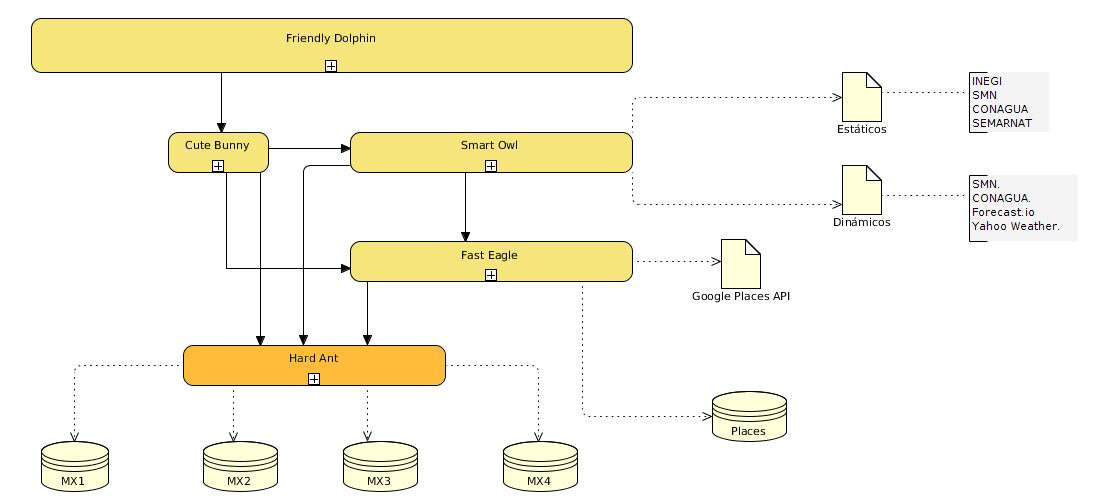
\includegraphics[width=\textwidth]{./images/DiagramaAmbienta2MX_HardAnt.png}
        \caption{Hard Ant, Módulo de Ambienta2MX.}
    \end{figure}
    \paragraph{Como complemento a la arquitectura, también contará con el proceso del registro masivo de información, exponiendo servicios que el módulo Smart Owl usará de forma constante para persistir la información estandarizada de diversas fuentes de información.}
    \paragraph{Hard Ant tiene como objetivo brindar los canales de acceso a las bases MX definidas en el diagrama general mediante servicios HTTP, estos servicios cumplen con la tarea de inserción y extracción de la información. }
    \paragraph{Este módulo es lo que sería considerado la capa del modelo de datos en un patrón MVC, ya que es la que tiene contacto de forma directa con los datos almacenados en las bases de datos orientadas a documentos gestionadas por Mongo.}
  \subsubsection{Alcances}
    \paragraph{Hard Ant fue diseñado para poder satisfacer la demanda en las cuatro bases de datos distrubidas, contando con un índice que se encarga de enviar la consulta a una base definda con base en la ubicación que le proporciona Fast Eagle.}
    \paragraph{Éste módulo también cuenta con la tarea de la generación de archivos de tipo CSV y JSON, que pueden ser utilizados para los fines que el usuario requiera. Todos los accesos realizarán mediante servicios de tipo REST siguiendo una Convención sobre configuración.} 
    \paragraph{Se utilizará un pool de conexiones a la base para garantizar el acceso o escritura a los datos además de brindar la posibilidad de respuestas asincronas y no bloqueantes entre las consultas realizadas.}
  \subsubsection{Restricciones}
    \paragraph{Para nuestro caso de estudio sólo se toma la información de la base de MX4, debido a que es la que contiene la información del Distrito Federal. Una de las limitantes más grandes es el consumo de memoria para la generación de archivos ya qué en principio se guardan de forma temporal y luego son enviados al cliente. La infraestructura que estamos manejando es limitada en recursos debido a que es gratuita.}
  \subsubsection{Arquitectura}
    \paragraph{A continuación se mostrará el de clases que define la estructura de Hard Ant.}
      \begin{figure}[b!]
        \centering
        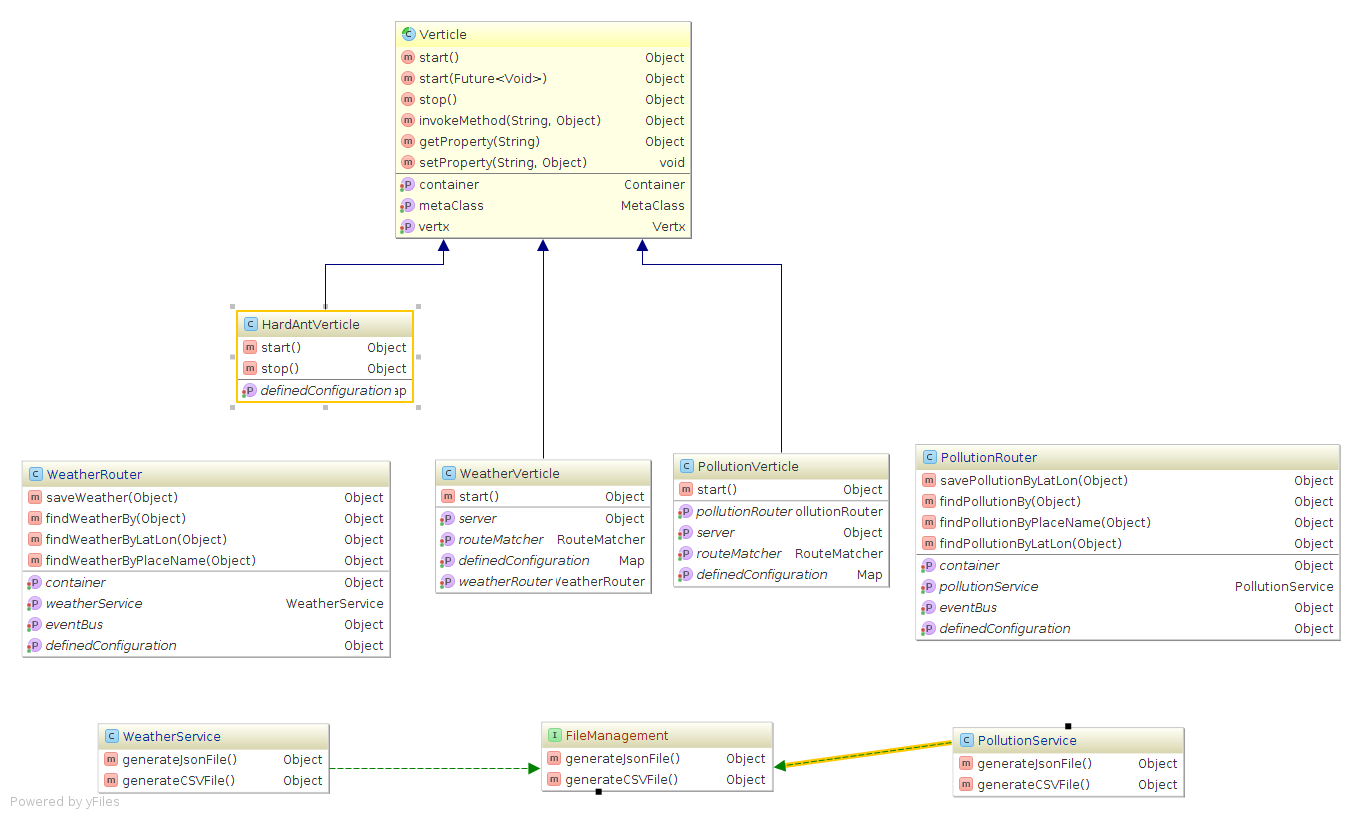
\includegraphics[width=\textwidth]{./images/HardAntClassDiagram.png}
        \caption{Diagrama de clases de Hard Ant}
      \end{figure}
    \paragraph{Las clases mostradas se ven reflejadas en el uso y adaptación de ``Verticles'', que son los componentes que se encargarán de atender peticiones, ya sea vía servicios REST o por comunicación mediante canales (Sockets), cómo se muestra en el siguiente diagrama a bloques.}
      \begin{figure}[b!]
        \centering
        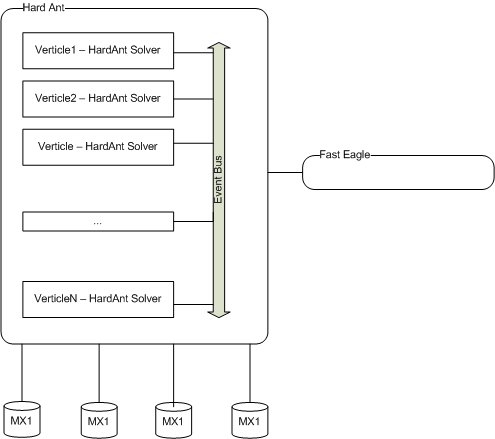
\includegraphics[width=\textwidth]{./images/DiagramaHardAnt.png}
        \caption{Diagrama a bloques de Hard Ant}
      \end{figure}
    \paragraph{En el diagrama se puede apreciar la replicación de ``Verticles'' que interactuan a través del mismo canal de información, esto brinda disponibilidad del servicio ya que las peticiones son atendidas y procesadas no sólo por un elemento existente si no varios. La interacción con este servicio se realizará utilizando servicios REST, utilizando el módulo de Cute Bunny como medio de comunicación con la vista que tendrá el usuario final.}
    \paragraph{Considerando trabajos más pesados (Obtención de datos climáticos considerando un radio, cadena de búsqueda o bien información de un punto definido) se utilizarán procesos en segundo plano, esto es posible gracias a la implementación de ``Verticles'' nativas de Vert.x, tecnología que será usada para el desarrollo y despliegue final de éste módulo.}
    \paragraph{Actualmente se propone el despliegue de varias ``Verticles'', además de las que el mismo framework despliega para el consumo de las bases de datos \cite{33}.Quedando en ocho, cuatro encargadas de la comunicación y distribución de la información y las cuatro restantes para atender peticiones.} 
    \paragraph{De forma específica, también se hará uso de los canales implementados por Vert.x para generar una comunicación con las bases de datos con la finalidad de poder generar la distribución de estas. Los canales podrían ser accedidos siempre y cuando se pertenezca a la misma red o bien al cluster de Vert.x, esta modalidad no ha sido habilitada por cuestiones de seguridad.}
  \subsubsection{Factibilidad} 
    \paragraph{Considerando el mismo modo de trabajo que en }
  \subsubsection{Implementación}
    \paragraph{Hablando más a detalle, Hard Ant, puede ser desplegado utilizando la línea de comandos gracias a las funciones que nos provee Gradle, framework utilizado para el maquetado, resolución de dependencias y gestión de tareas del proyecto. \cite{34}}
    \paragraph{El código y el proyecto como tal se encuentran en línea utilizando Git\cite{38} en conjunto con Github\cite{39}, para el proceso de control de versiones. Para la gestión de tareas y desarrollo del proyecto fue utilizado Gradle en conjunton con Vert.x.}
    \paragraph{Las ventajas que nos ofrece Git/Github es la integración con procesos de desarrollo utilizando metodologías ágiles. La siguiente imagen muestra el control y manejo de issues (análogos a objetivos o features) que fueron desarrollados para cumplir con los objetivos y mejoras planteadas para cada módulo.}
    \begin{figure}[h!]
        \centering
          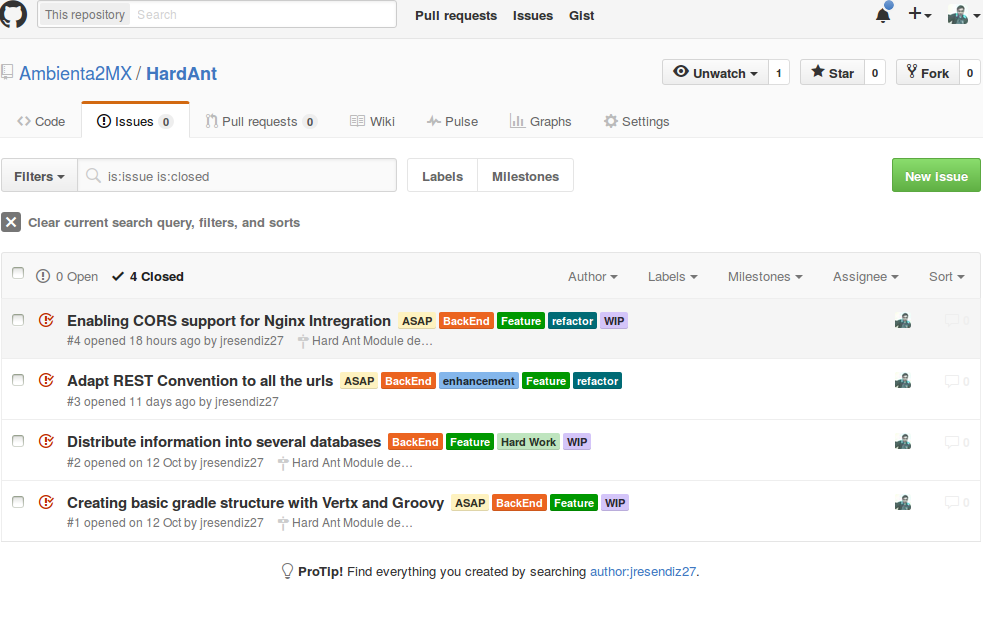
\includegraphics[width=\textwidth]{./images/HardAntIssues.png}
          \caption{Hard Ant, Integración con Github.}
    \end{figure}
    \paragraph{Este módulo se puede encontrar en cualquier otra máquina, debido al método de comunicación utilizado entre los módulos, sólo basta con realizar la configuración de las direcciones o dominios donde se encuentra alojado para qué este puede pueda ser accedido.}
  \subsubsection{Pruebas y Capturas de pantalla}
    \paragraph{A continuación se muestran algunas pruebas realizadas y las capturas de pantalla del servicio REST y la respuesta qué este nos regresa.}
      \begin{figure}[h!]
        \centering
          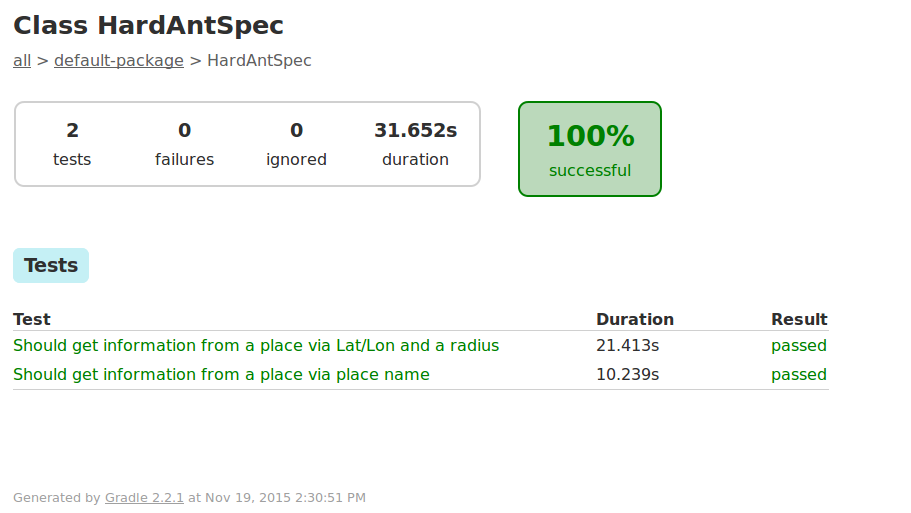
\includegraphics[width=\textwidth]{./images/PruebasHardAnt}
          \caption{Hard Ant, Pruebas unitarias.}
      \end{figure}
      \begin{figure}[h!]
        \centering
          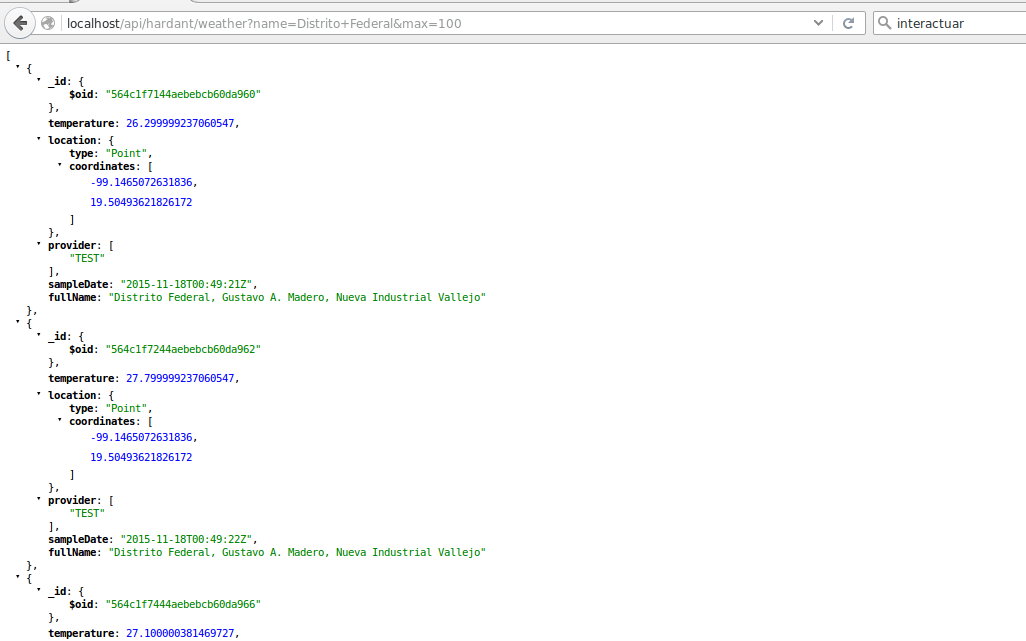
\includegraphics[width=\textwidth]{./images/CapturaHardAnt}
          \caption{Hard Ant, Respuesta del servicio rest.}
      \end{figure}